\documentclass[10pt,a4paper]{article}
\usepackage[left=2cm,right=2cm,top=2cm,bottom=2cm]{geometry}
\usepackage[T1]{fontenc}
\usepackage{lmodern}
\usepackage[spanish,es-tabla,es-noquoting]{babel}
\usepackage[dvipsnames]{xcolor}
\usepackage[fleqn]{mathtools}
\usepackage{booktabs}
\usepackage{amsmath}
\usepackage{latexsym}
\usepackage{graphicx}
\usepackage{nccmath}
\usepackage{multicol}
\usepackage{listings}
\usepackage{color}
\usepackage{float}
\usepackage{csquotes}

\definecolor{colorIPN}{rgb}{0.5, 0.0,0.13}
\definecolor{colorESCOM}{rgb}{0.0, 0.5,1.0}
\graphicspath{ {imagenes/} }

\begin{document}
%#########################################################
\begin{titlepage}
	\centering

	{\color{colorIPN}\rule{\linewidth}{1.4pt}}\\[0.35cm]
	{\scshape\LARGE Instituto Politécnico Nacional}\\[0.2cm]
	{\scshape\Large \color{colorESCOM}Escuela Superior de Cómputo}\\[0.35cm]
	{\color{colorIPN}\rule{\linewidth}{0.5pt}}

	\vspace{1.6cm}
	{\large \color{colorESCOM}\MakeUppercase{Administración de Servicios en Red}\par}

	\vspace{2cm}
	\noindent
	\begin{minipage}[t]{0.025\linewidth}
		\color{colorESCOM}\rule{3.2pt}{3.6cm}
	\end{minipage}%
	\hspace{0.5cm}%
	\begin{minipage}[t]{0.87\linewidth}
		\raggedright\huge\bfseries\color{colorIPN} Enrutamiento estático
	\end{minipage}

	\vspace{2.8cm}
	\renewcommand{\arraystretch}{1.7}
	\begin{tabular}{r @{\hspace{0.6cm}} l}
		{\bfseries\color{colorESCOM}Profesor:} & {\itshape\color{colorIPN} Marco Antonio Tenorio Marrón} \\
		{\bfseries\color{colorESCOM}Alumno:}   & {\itshape\color{colorIPN} Angel Frausto Robles} \\
		{\bfseries\color{colorESCOM}Boleta:}   & {\itshape\color{colorIPN} 2019630177} \\
		{\bfseries\color{colorESCOM}Grupo:}    & {\itshape\color{colorIPN} 7CM3} \\
	\end{tabular}

	\vfill
	{\color{colorIPN}\rule{0.25\linewidth}{0.5pt}}\\[0.25cm]
	{\small\color{colorIPN}\today\par}
	\vspace{1cm}
\end{titlepage}

\renewcommand\lstlistingname{Código}

\lstset{
	basicstyle=\small\ttfamily,
	numbers=left,
	numberstyle=\tiny,
	frame=tb,
	tabsize=4,
	columns=fixed,
	showstringspaces=false,
	showtabs=false,
	keepspaces,
	commentstyle=\color{Violet},
	keywordstyle=\color{colorIPN} \bfseries,
	stringstyle=\color{colorESCOM},
	breaklines=true,
	extendedchars=true,
	inputencoding=utf8,
	literate=
		{á}{{\'a}}1 {é}{{\'e}}1 {í}{{\'i}}1 {ó}{{\'o}}1 {ú}{{\'u}}1
		{Á}{{\'A}}1 {É}{{\'E}}1 {Í}{{\'I}}1 {Ó}{{\'O}}1 {Ú}{{\'U}}1
		{ñ}{{\~n}}1 {Ñ}{{\~N}}1 {ü}{{\"u}}1 {¿}{{?`}}1 {¡}{{!`}}1
}

\pagenumbering{arabic}

%################################################
\section{\color{colorIPN}{Objetivo}}

Configurar el direccionamiento IP y las rutas estáticas de tres routers (R1, R2 y R3) para que los cuatro equipos finales, distribuidos en tres redes distintas, puedan comunicarse entre sí, y comprobar la conectividad con \texttt{ping} desde las computadoras virtuales.

%################################################
\section{\color{colorIPN}{Topología}}

La topología forma un triángulo de routers. R1 atiende la RED 1 a través de un switch, y R2 y R3 atienden una red con un equipo cada uno. Los tres routers se enlazan entre sí con redes punto a punto /30:

\begin{figure}[H]
	\centering
	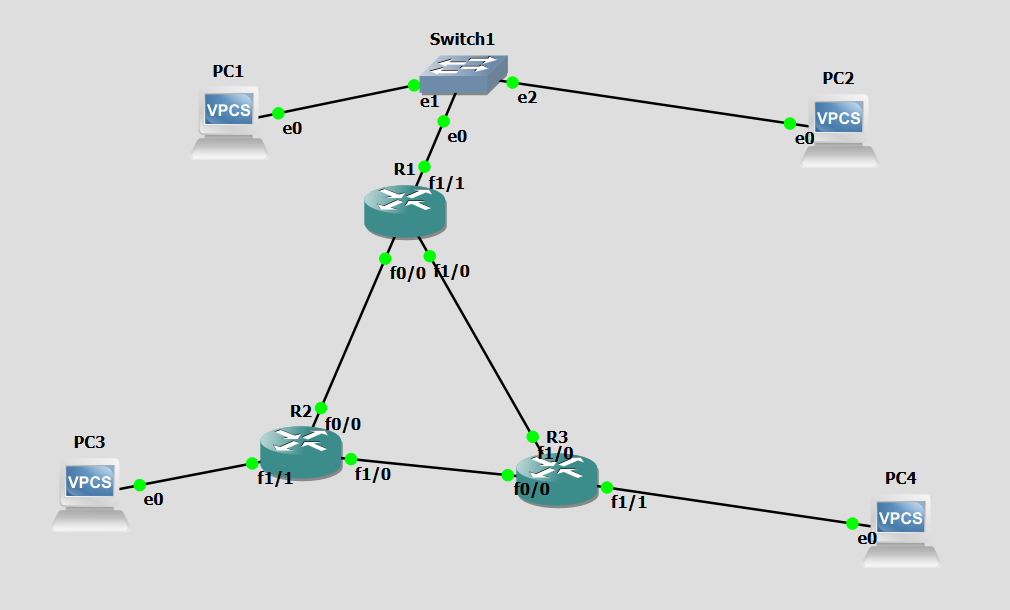
\includegraphics[width=0.85\linewidth]{00_topologia.png}
	\caption{Topología en GNS3 con todos los dispositivos en ejecución}
	\label{img:topologia}
\end{figure}

\begin{table}[H]
	\centering
	\begin{tabular}{@{}lllll@{}}
		\toprule
		Red & Dirección de red & Dispositivo & Interfaz & Dirección IP \\
		\midrule
		RED 1 & 192.100.10.0/24 & R1 & f1/1 & 192.100.10.1 \\
		      &                 & PC1 & e0 & 192.100.10.100 \\
		      &                 & PC2 & e0 & 192.100.10.101 \\
		RED 2 & 192.100.15.0/24 & R2 & f1/1 & 192.100.15.1 \\
		      &                 & PC3 & e0 & 192.100.15.100 \\
		RED 3 & 192.100.20.0/24 & R3 & f1/1 & 192.100.20.1 \\
		      &                 & PC4 & e0 & 192.100.20.100 \\
		\midrule
		R1--R2 & 10.10.0.0/30 & R1 / R2 & f0/0 / f0/0 & 10.10.0.1 / 10.10.0.2 \\
		R2--R3 & 10.10.0.4/30 & R2 / R3 & f1/0 / f0/0 & 10.10.0.5 / 10.10.0.6 \\
		R3--R1 & 10.10.0.8/30 & R3 / R1 & f1/0 / f1/0 & 10.10.0.9 / 10.10.0.10 \\
		\bottomrule
	\end{tabular}
	\caption{Direccionamiento de la topología}
	\label{tab:direccionamiento}
\end{table}

Los enlaces entre routers usan máscara /30 (255.255.255.252): una red punto a punto solo necesita dos direcciones útiles, una por cada extremo.

%################################################
\section{\color{colorIPN}{Desarrollo}}

\subsection{\color{colorESCOM}{Configuración de los routers}}

Cada router conoce por sí solo únicamente las redes a las que está conectado. Para alcanzar las demás se agregó una \textbf{ruta estática} con \texttt{ip route \textit{red máscara siguiente-salto}} por cada red remota: las dos redes de equipos finales y el enlace /30 que no toca directamente. Así cada router tiene tres rutas estáticas y su tabla queda completa.

\begin{lstlisting}[language=bash, caption={Configuración de R1}]
enable
configure terminal
hostname R1
interface FastEthernet1/1
 ip address 192.100.10.1 255.255.255.0
 no shutdown
interface FastEthernet0/0
 ip address 10.10.0.1 255.255.255.252
 no shutdown
interface FastEthernet1/0
 ip address 10.10.0.10 255.255.255.252
 no shutdown
exit
ip route 192.100.15.0 255.255.255.0 10.10.0.2
ip route 192.100.20.0 255.255.255.0 10.10.0.9
ip route 10.10.0.4 255.255.255.252 10.10.0.2
end
write memory
\end{lstlisting}

\begin{lstlisting}[language=bash, caption={Configuración de R2}]
enable
configure terminal
hostname R2
interface FastEthernet1/1
 ip address 192.100.15.1 255.255.255.0
 no shutdown
interface FastEthernet0/0
 ip address 10.10.0.2 255.255.255.252
 no shutdown
interface FastEthernet1/0
 ip address 10.10.0.5 255.255.255.252
 no shutdown
exit
ip route 192.100.10.0 255.255.255.0 10.10.0.1
ip route 192.100.20.0 255.255.255.0 10.10.0.6
ip route 10.10.0.8 255.255.255.252 10.10.0.1
end
write memory
\end{lstlisting}

\begin{lstlisting}[language=bash, caption={Configuración de R3}]
enable
configure terminal
hostname R3
interface FastEthernet1/1
 ip address 192.100.20.1 255.255.255.0
 no shutdown
interface FastEthernet0/0
 ip address 10.10.0.6 255.255.255.252
 no shutdown
interface FastEthernet1/0
 ip address 10.10.0.9 255.255.255.252
 no shutdown
exit
ip route 192.100.10.0 255.255.255.0 10.10.0.10
ip route 192.100.15.0 255.255.255.0 10.10.0.5
ip route 10.10.0.0 255.255.255.252 10.10.0.10
end
write memory
\end{lstlisting}

\subsection{\color{colorESCOM}{Configuración de las PCs (VPCS)}}

Cada PC es un nodo VPCS y se configura con su IP, máscara y puerta de enlace (la interfaz del router de su red) en un solo comando, que después se guarda con \texttt{save}:

\begin{lstlisting}[language=bash, caption={Configuración de las cuatro PCs}]
PC1> ip 192.100.10.100 255.255.255.0 192.100.10.1
PC2> ip 192.100.10.101 255.255.255.0 192.100.10.1
PC3> ip 192.100.15.100 255.255.255.0 192.100.15.1
PC4> ip 192.100.20.100 255.255.255.0 192.100.20.1
\end{lstlisting}

%################################################
\section{\color{colorIPN}{Evidencias}}

\subsection{\color{colorESCOM}{Tabla de interfaces y tabla de ruteo de cada router}}

La tabla de interfaces se obtuvo con \texttt{show ip interface brief | exclude unassigned}, que oculta las interfaces sin dirección. Las tres interfaces de cada router están en estado \texttt{up/up}. En la tabla de ruteo (\texttt{show ip route}) las rutas marcadas con \textbf{C} son las directamente conectadas y las marcadas con \textbf{S} son las estáticas.

\begin{figure}[H]
	\centering
	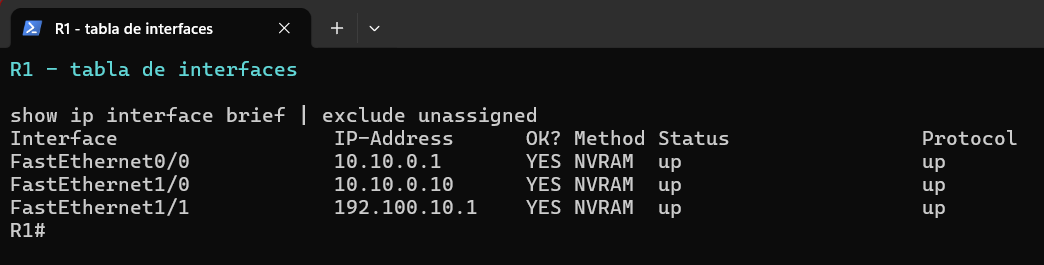
\includegraphics[width=0.8\linewidth]{01a_R1_interfaces.png}\\[0.4cm]
	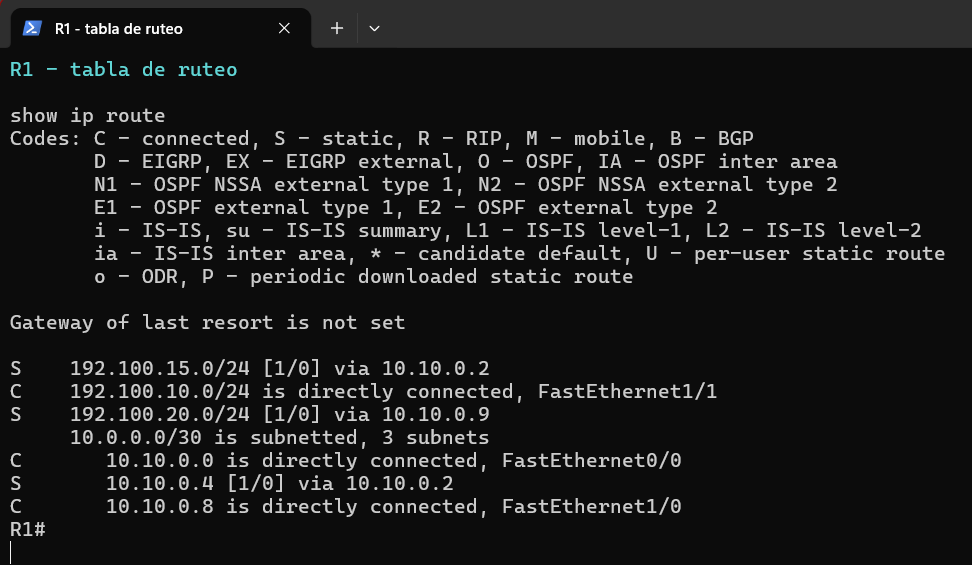
\includegraphics[width=0.8\linewidth]{01b_R1_ruteo.png}
	\caption{R1: tabla de interfaces y tabla de ruteo}
	\label{img:r1}
\end{figure}

\begin{figure}[H]
	\centering
	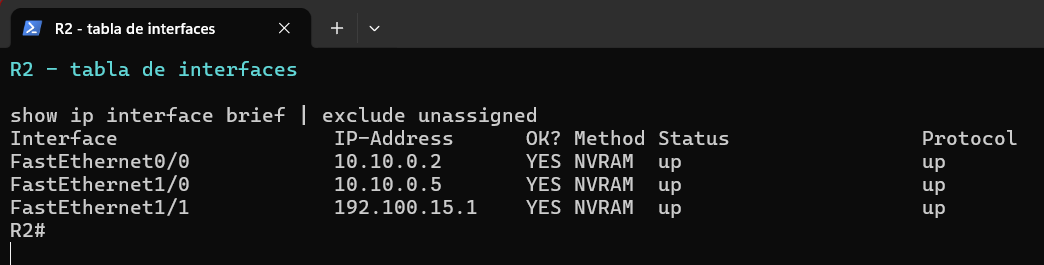
\includegraphics[width=0.8\linewidth]{02a_R2_interfaces.png}\\[0.4cm]
	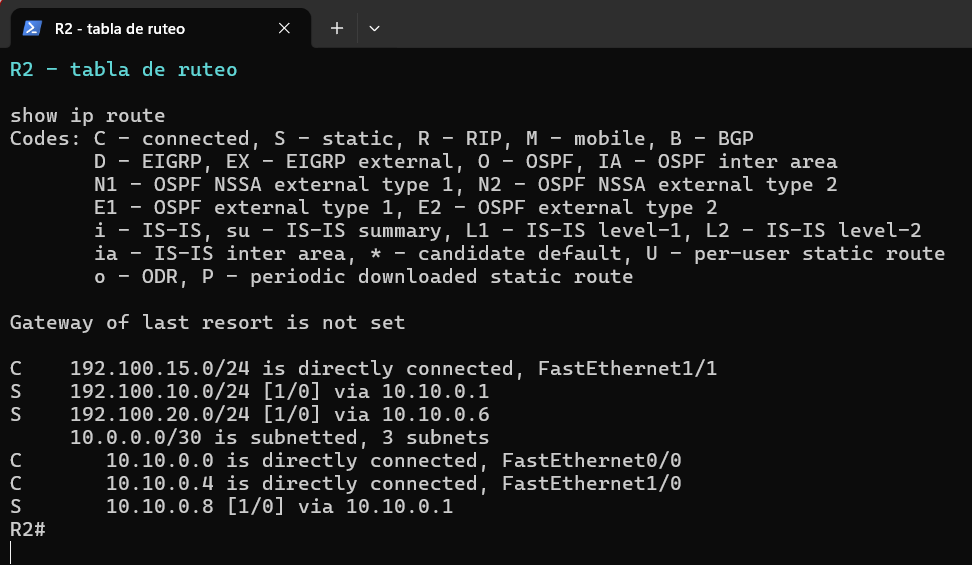
\includegraphics[width=0.8\linewidth]{02b_R2_ruteo.png}
	\caption{R2: tabla de interfaces y tabla de ruteo}
	\label{img:r2}
\end{figure}

\begin{figure}[H]
	\centering
	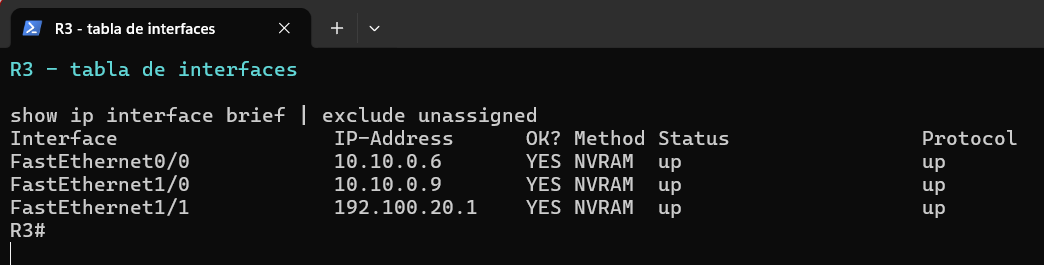
\includegraphics[width=0.8\linewidth]{03a_R3_interfaces.png}\\[0.4cm]
	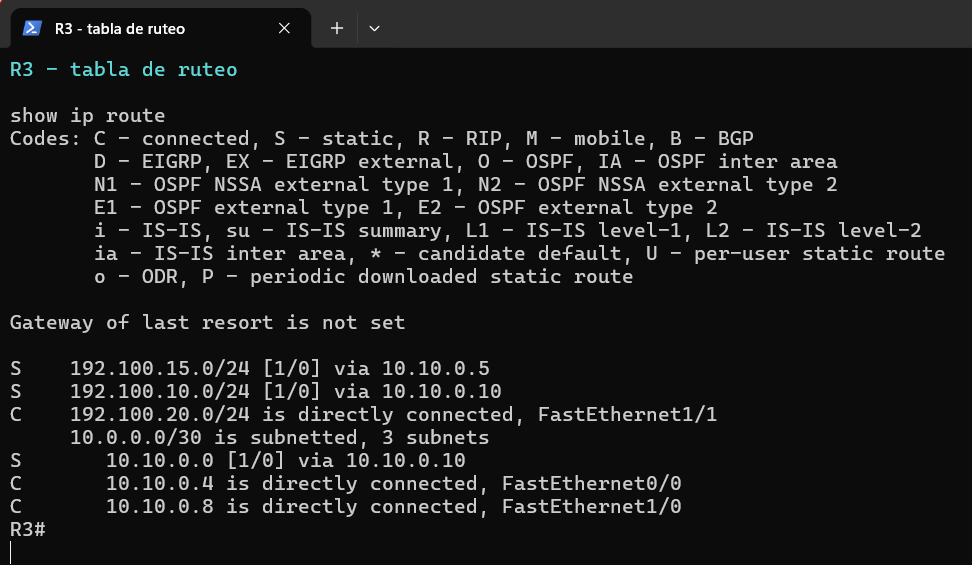
\includegraphics[width=0.8\linewidth]{03b_R3_ruteo.png}
	\caption{R3: tabla de interfaces y tabla de ruteo}
	\label{img:r3}
\end{figure}

\subsection{\color{colorESCOM}{Configuración de cada PC}}

\begin{figure}[H]
	\centering
	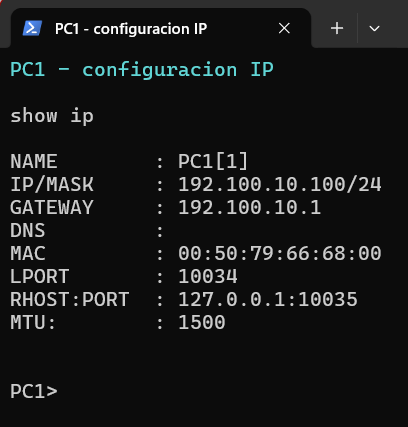
\includegraphics[width=0.24\linewidth]{04_PC1_config.png}\hfill
	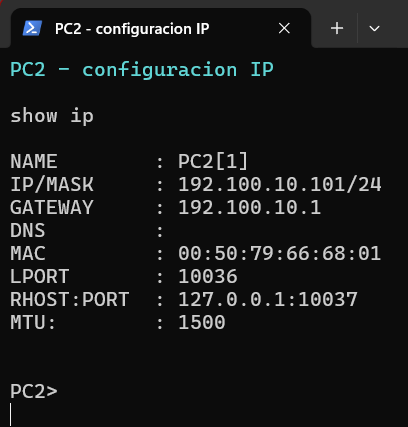
\includegraphics[width=0.24\linewidth]{05_PC2_config.png}\hfill
	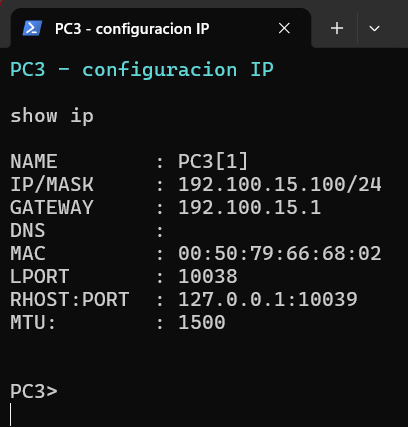
\includegraphics[width=0.24\linewidth]{06_PC3_config.png}\hfill
	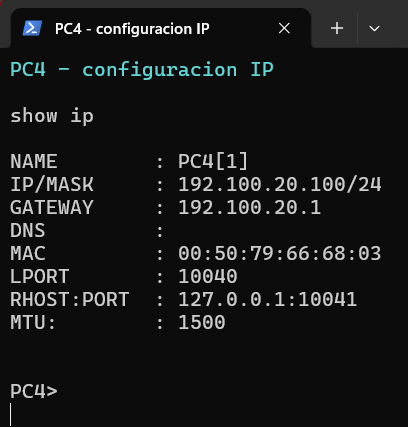
\includegraphics[width=0.24\linewidth]{07_PC4_config.png}
	\caption{Comando \texttt{show ip} en PC1, PC2, PC3 y PC4 (de izquierda a derecha)}
	\label{img:pcs}
\end{figure}

\subsection{\color{colorESCOM}{Prueba de comunicación entre los equipos finales}}

Se probó \texttt{ping} entre las seis parejas posibles de equipos finales. Los pings entre redes distintas llegan con \texttt{ttl=62}: el paquete sale con TTL 64 y cada router que atraviesa le resta 1, así que llegó a través de dos routers. El ping entre PC1 y PC2, que están en la misma red y solo pasan por el switch, llega con \texttt{ttl=64}.

Antes de cada captura se ejecutó el mismo \texttt{ping} una vez sin mostrarlo, para que la caché ARP estuviera poblada. En una prueba en frío, el primer paquete se pierde mientras se resuelve el ARP, y por eso las capturas muestran los cinco paquetes respondidos.

\begin{figure}[H]
	\centering
	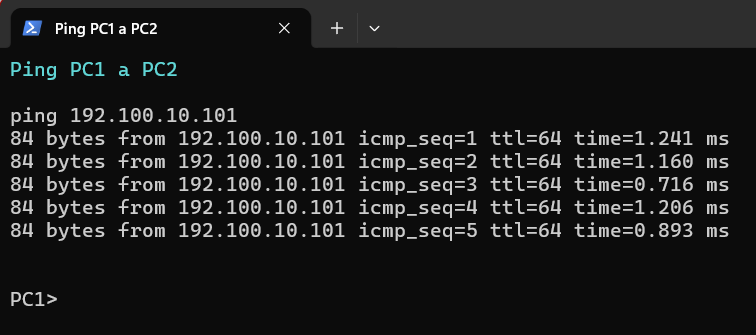
\includegraphics[width=0.48\linewidth]{08_ping_PC1_PC2.png}\hfill
	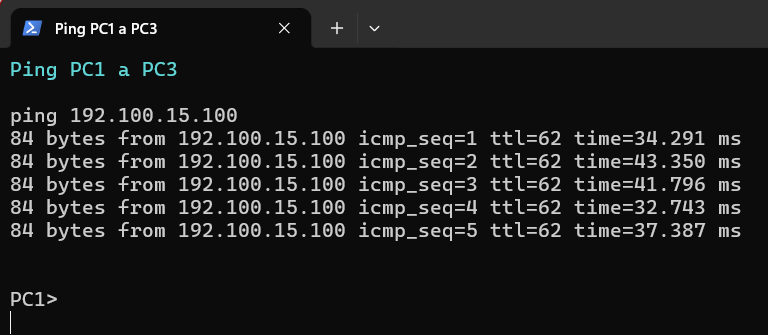
\includegraphics[width=0.48\linewidth]{09_ping_PC1_PC3.png}
	\caption{PC1 a PC2 (misma red) y PC1 a PC3}
	\label{img:ping1}
\end{figure}

\begin{figure}[H]
	\centering
	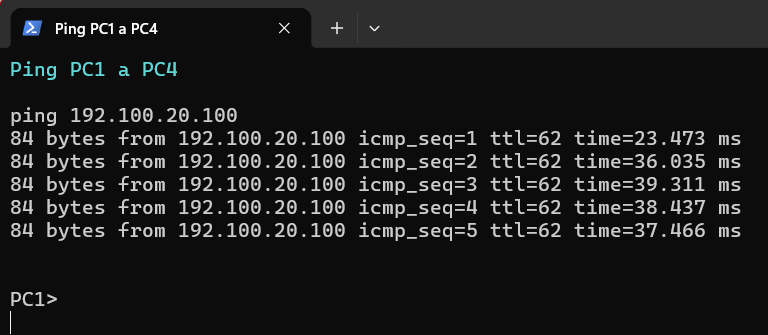
\includegraphics[width=0.48\linewidth]{10_ping_PC1_PC4.png}\hfill
	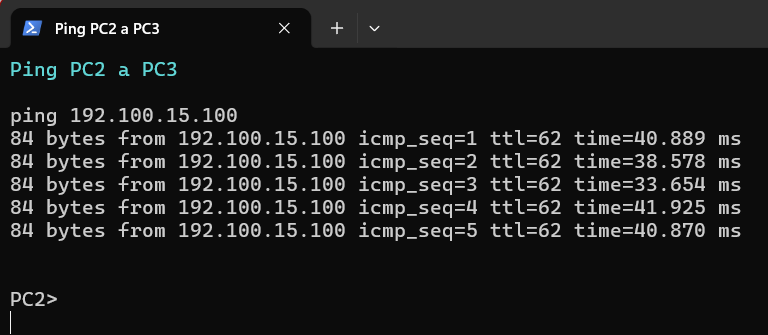
\includegraphics[width=0.48\linewidth]{11_ping_PC2_PC3.png}
	\caption{PC1 a PC4 y PC2 a PC3}
	\label{img:ping2}
\end{figure}

\begin{figure}[H]
	\centering
	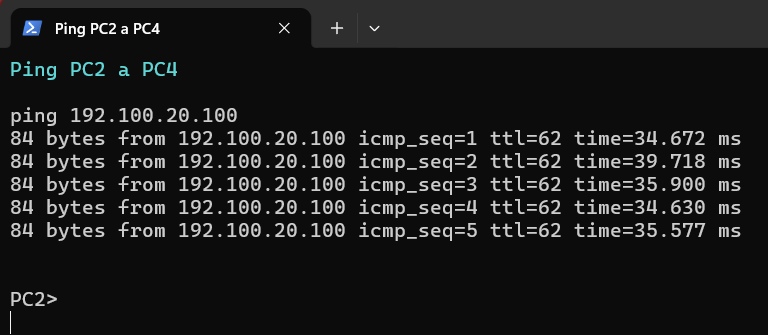
\includegraphics[width=0.48\linewidth]{12_ping_PC2_PC4.png}\hfill
	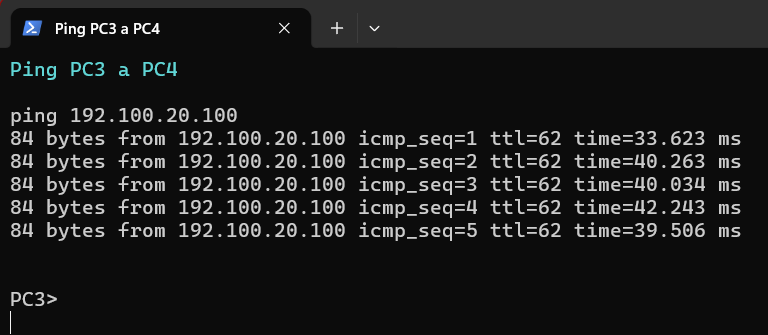
\includegraphics[width=0.48\linewidth]{13_ping_PC3_PC4.png}
	\caption{PC2 a PC4 y PC3 a PC4}
	\label{img:ping3}
\end{figure}

%################################################
\section{\color{colorIPN}{Conclusiones}}

Las cuatro PCs se comunican entre sí a través de los tres routers usando únicamente rutas estáticas. Con solo las direcciones IP, cada router conoce sus redes directamente conectadas y nada más, así que fue necesario declarar a mano cada red remota y su siguiente salto. La ventaja del ruteo estático es que es sencillo y predecible, y por eso las tablas de ruteo de esta práctica se pueden leer y verificar una por una. Su desventaja es que no se adapta a los cambios: si se agrega una red o se cae un enlace, hay que modificar la configuración de cada router afectado, y ese mantenimiento manual crece con el tamaño de la red.

\end{document}
